\chapter{Source and Boundary Conditions}\label{chap.source}

\section{Radial Domain and Boundary Conditions}\label{sec.boundary}

GYRO has the option of treating periodic (variously called flux-tube, 
or local) or nonperiodic (global) boundary conditions on 
$(\dphin,\dapn,h_{\sigma,n})$.

\begin{equation}
r_i = \bar{r} - \frac{L}{2} + \Delta r (i-1) 
\quad\text{for}\quad i = 1,\ldots,n_r \; .
\end{equation}
where 
%
\begin{equation}
\Delta r \doteq 
\begin{cases}
 \displaystyle L/n_r & \text{periodic; \param{BOUNDARY\_METHOD=1}} \; ,\\
 \displaystyle L/(n_r-1) & \text{nonperiodic; \param{BOUNDARY\_METHOD=2}} \; .
\end{cases} 
\end{equation}

\noindent
The central radius, $\bar{r}$, is specified by the INPUT 
parameter \param{RADIUS}.

\subsection{Periodic}

Flux-tube boundary conditions effectively eliminate the inner 
and outer radial boundaries by making the quantities periodic in $r$.  
For example, 
%
\begin{equation}
\dphi_n(r_1,\theta) = \dphi_n(r_{n_r},\theta) \; .
\end{equation}

\noindent
Use of this boundary condition is very useful for 
local linear analyses (all the linear results presented 
in this report use flux-tubes) and computationally 
efficient for restricted nonlinear studies.  However, 
the flux-tube mode of operation is incompatible with 
variation of the equilibrium profiles.

\subsection{Nonperiodic}

In order to study physical effects associated with profile 
variation, it is necessary to abandon flux-tubes and use 
some type of nonperiodic radial boundary condition.  In the 
design of nonperiodic end conditions, we have attempted to 
minimize as much as possible the effect of the boundaries 
on the interior dynamics.  To this extent, our goal was 
to construct ``benign'' rather than physical end conditions.
First, to make the notation less cumbersome, let us write
%
\begin{align}
r_a &~\rightarrow r_1 \; , \\
r_a^{\rm buffer} &~\rightarrow r_p \; , \\
r_b^{\rm buffer} &~\rightarrow r_{n_r-p+1} \; , \\
r_b &~\rightarrow r_{n_r} \; , 
\end{align}

\noindent
where the width of the buffer region, $p$, is set by the input 
parameter \param{EXPLICIT\_DAMP\_GRID}.

First, at the extreme edges of the computational domain, $r=r_a$ 
and $r=r_b$, we impose Dirichlet boundary conditions on all 
toroidal harmonics.
%
\begin{align}
\hn(r_a,\theta) = \dphi_n(r_a,\theta) = &~0 \; , \\
\hn(r_b,\theta) = \dphi_n(r_b,\theta) = &~0 \; .
\end{align}

\begin{figure}
\begin{center}
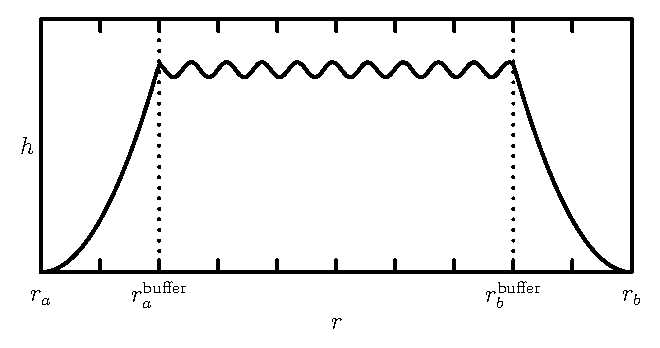
\includegraphics[scale=1.0]{figures/boundary.eps}
\caption{Illustration of placement of boundary {\it buffer} regions.}
\label{fig.boundary}
\end{center}
\end{figure}

\noindent
Experience shows that these boundary conditions, in the 
absence of any other tricks, will give rise to strong 
oscillations at the boundaries.  The effect of these 
oscillations will be felt well into the interior of the 
computational domain and so various techniques were 
explored in an effort to mitigate the corruption of the 
interior solution.  One solution that works well is the 
imposition of a ``buffer'' region; that is, a region 
near the boundary where we impose an explicit damping 
on the $n=0$ evolution equation.  Generally speaking, we 
modify the normalized gyrokinetic equation, Eq.~(\ref{eq.hnnorm}),
according to
%
\begin{equation}
\frac{\partial h_{\sigma,0}}{\partial\hat{t}} 
 = \rhs_0-\frac{a \nu_\sigma(r)}{\bar{c}_s}\, H_{\sigma,0} \; ,
\end{equation}

\noindent
where
\begin{equation}
\nu_\sigma(r) \doteq
\begin{cases}
\nu_\sigma^{\rm buffer} &
 \text{if $r_a \le r \le r_a^{\rm buffer}$} \; , \\
0 & 
 \text{if $r_a^{\rm buffer} < r < r_b^{\rm buffer}$} \; , \\
\nu_\sigma^{\rm buffer} &
 \text{if $r_b^{\rm buffer} \le r \le r_b$} \; . 
\end{cases}
\end{equation}

\noindent
An illustration of the effect of this technique on 
computed fields is given in Fig.~\ref{fig.boundary}.
In GYRO, the strength of the damping in the buffer is controlled 
by the following INPUT parameters 
%
\begin{align}
\param{EXPLICIT\_DAMP} 
  \rightarrow \frac{a \nu_i^{\rm buffer}}{\bar{c}_s} \; , \\
\param{EXPLICIT\_DAMP\_ELECTRON} 
  \rightarrow \frac{a \nu_e^{\rm buffer}}{\bar{c}_s} \; .
\end{align}

%-----------------------------------------------------------------
\section{Long-wavelength Source}

One dramatic benefit of flux-tube simulations is that no 
special techniques are required to keep the equilibrium from
evolving.  In this case, the equilibrium is analytically 
separable from the fluctuations and there is no coupling 
between them.  In a global simulation there is no such 
possibility for separability and short-wavelength radial
fluctuations are coupled to long-wavelength equilibrium-scale 
dynamics.  In this note we propose a method to partially 
decouple equilibrium from fluctuations so as to keep the 
equilibrium profiles from changing.

\subsection{Formulation of the problem}

\noindent
As in the previous section, we write the $n=0$ component 
of the gyrokinetic equation for fluctuations as
%
\begin{equation}
\frac{\partial h_{\sigma,0}}{\partial \hat{t}} = \rhs_0(r) \; .
\end{equation}

\noindent
If the system were periodic in $r$, we could write the Fourier 
space expression
%
\begin{equation}
\frac{\partial \widetilde{h}_p}{\partial\hat{t}} = \widetilde{\rhs}_p \; ,
\end{equation}

\noindent
where 
%
\begin{equation}
h_{\sigma,0}(r) = \sum_p \widetilde{h}_p \, e^{- 2 \pi i p r/L} \; .
\end{equation}

\noindent
Then, in a flux-tube simulation, we would simply set 
$\widetilde{h}_0=0$, which corresponds to zero radial 
average of the $n=0$ fluctuations.  Since the $p=0$ 
equations decouples from the rest of the problem (the 
$p=0$ component of the $\exb$ nonlinearity is identically 
zero), this is allowed.  However, in a global simulation, 
there is no way to cleanly separate the equilibrium from the 
fluctuations, because there is no exact analogue of 
$\widetilde{h}_0$.

\subsection{Solution by damping}

Instead of ignoring $p=0$ as in a flux-tube simulation, 
we can instead damp the long-wavelength components. This 
will drain, in a nonconservative fashion, any pumping that 
the equilibrium-scale distribution receives from nonlinear 
coupling. In real space, then, we modify the gyrokinetic 
equation according to
%
\begin{equation}
\frac{\partial h_{\sigma,0}}{\partial\hat{t}} 
 = \rhs_0 - \frac{a \nu_{\rm source}}{\bar{c}_s} 
 \langle h_{\sigma,0} \rangle \; ,
\end{equation}
 
\noindent
where the angle brackets denote a projection onto long wavelengths 
only.  For example, 
%
\begin{equation}
 \langle h_{\sigma,0}(r) \rangle = 
  \sum_{p=1}^{\param{N\_SOURCE}+4} c_p F_p(r) \; .
\end{equation}

\begin{figure}
\begin{center}
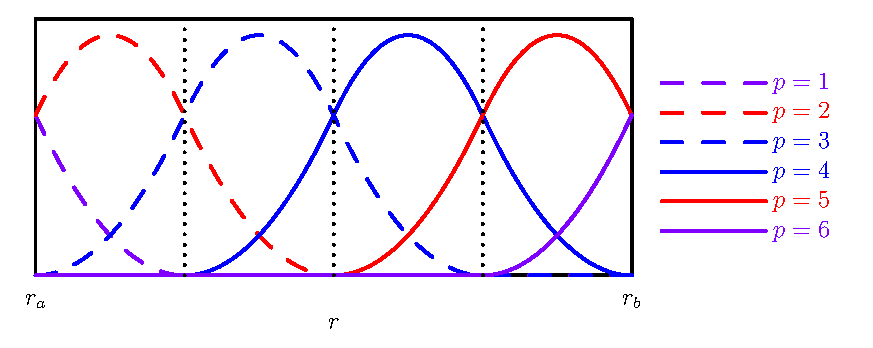
\includegraphics[scale=1.0]{figures/source.eps}
\caption{Illustration of quadratic finite-element basis for
  \param{N\_SOURCE=2}.  Note that $p=1,2$ and $p=5,6$ are 
partial elements.}
\label{fig.source}
\end{center}
\end{figure}

\noindent
The expansion coefficients satisfy $M_{p\pp} c_{\pp} = S_p$ where
%
\begin{equation}
M_{p\pp} = \int_{r_a}^{r_b} dr \, F_p(r) F_{\pp}(r) 
\quad\mbox{and}\quad
S_p = \int_{r_a}^{r_b} dr \,h_{\sigma,0}(r) F_p(r) \; . 
\end{equation}
In GYRO, we take the $F_p$ to be quadratic finite elements.  These 
are defined as scaled translates of the function $N^{(3)}$ given in 
Eq.~(\ref{eq.quadraticfe}).  We also include partial elements in
order to satisfy {\it general nonperiodic boundary conditions}, 
rather than Dirichlet boundary conditions.  The reason for doing this 
is to most gracefully accomodate the rapid variation of $h$ in 
the buffer regions. The choice of \param{N\_SOURCE} is somewhat 
arbitrary but should be small enough to hold only the longest 
wavelengths fixed (i.e., between 1 and 3).

Note that if the time rate of change is slow, $\partial_t \rightarrow 0$, 
and the steady-state solution for the long-wavelength component is 
%
\begin{equation}
 \langle h_{\sigma,0}(r) \rangle = 
  \langle \rhs_0\rangle /\nu_{\rm source} \; ,
\end{equation}

\noindent
which can be made arbitrarily small by increasing $\nu_{\rm source}$.
In GYRO, the strength of the source is controlled by  
%
\begin{equation}
\param{NU_\_SOURCE} 
  \rightarrow \frac{a \nu_{\rm source}}{\bar{c}_s} \; . 
\end{equation}

